% !TEX encoding = UTF-8 Unicode
% !TEX root = rapport.tex

\part{Conclusion}\label{conclu}

\chapter*{L'effet dominos}
Nous avons vu lors de la première partie que de tous temps les sociétés ont une certaine réticence aux innovations technologiques. Au niveau du système éducatif et de l'arrivée des ordinateurs personnels, cela a rapidement créé un décalage entre la société et les écoles. Ce décalage occasionne de nombreux troubles, comme la difficulté à l'insertion professionnelle, de nombreux échecs scolaires (distraction des élèves), voir de tragiques évènements comme le suicide de jeunes pris aux piège de la diffusion de contenus intimes via internet (voir seconde partie).

\chapter*{Concrètement}
Comment pourrions-nous améliorer le système éducatif concrètement ? Nous avons tenu à rappeler quelques points, certainement classés du plus simple au plus complexe à mettre en œuvre.

\begin{description}
  \item[Projets vs. Problèmes] : un élève ne sera naturellement pas impliqué dans la résolution d'un problème dont la correction est donnée 15 minutes plus tard. Ici nous proposons de regrouper et d'inclure ces problèmes dans des projets globaux, effectués en groupes pour favoriser les interactions, et cela sur plusieurs jours (de deux jours à une semaine).
  \item[Multi-niveaux] : bien que le découpage des classes par âge n'ait pas vraiment de sens face à un découpage par centres d'intérêts ou de compétences, nous comprenons bien difficulté de gestion administrative. C'est pourquoi nous proposons, tout en conservant cette répartition par âge, de ne plus voir les différents niveaux comme des frontières, afin de pouvoir organiser des projet mixtes multi-niveaux. Cela permettrait un enrichissement mutuel, notamment les plus jeunes apportent une vision nouvelle sur certains problèmes, et les plus âgés auront tendance à prendre le rôle d'encadrant et d'enseignant.
  \item[Multi-disciplinaires] : beaucoup de sujets regroupent en fait de nombreux domaines. L'idée de briser les frontières entre les disciplines permettrait la réalisation de projets extrêmement intéressants au travers de sujets transversaux en mêlant plusieurs enseignements voir sections ou cursus universitaires.
  \item[Concret avant Abstrait] : idée essentielle et facile à appliquer qui découle directement de la philosophie du contructionnisme : toujours confronter l'élève à la problématique avant de lui enseigner des problèmes concrets.
  \item[Investissement sur l'avenir] : le constat est simple, le système éducatif devrait faire comme le font les grandes entreprises en investissant sur l'avenir. Il serait certainement plus raisonnable d'effectuer des recherches pour développer de nouvelles méthodes d'éducation plutôt que de renouveler les parcs informatiques.
\end{description}

\chapter*{Vers les neurosciences\ldots}
Avant de clôturer ce rapport, nous souhaitons souligner le fait que d'autre méthodes d'apprentissages existent, notamment basées sur les neurosciences. En effet de réels progrès ont eu lieu dans ce domaine ces dix dernières années, ce qui a permis, grâces aux connaissances acquises sur le fonctionnement du cerveau, de mettre en place des exercices adaptés. Particulièrement, nous savons que la réalisation d'un résumé en fin de cours, de préférence sous la forme d'une carte mentale favorise grandement la mémorisation des leçons.

\begin{figure}[H]
  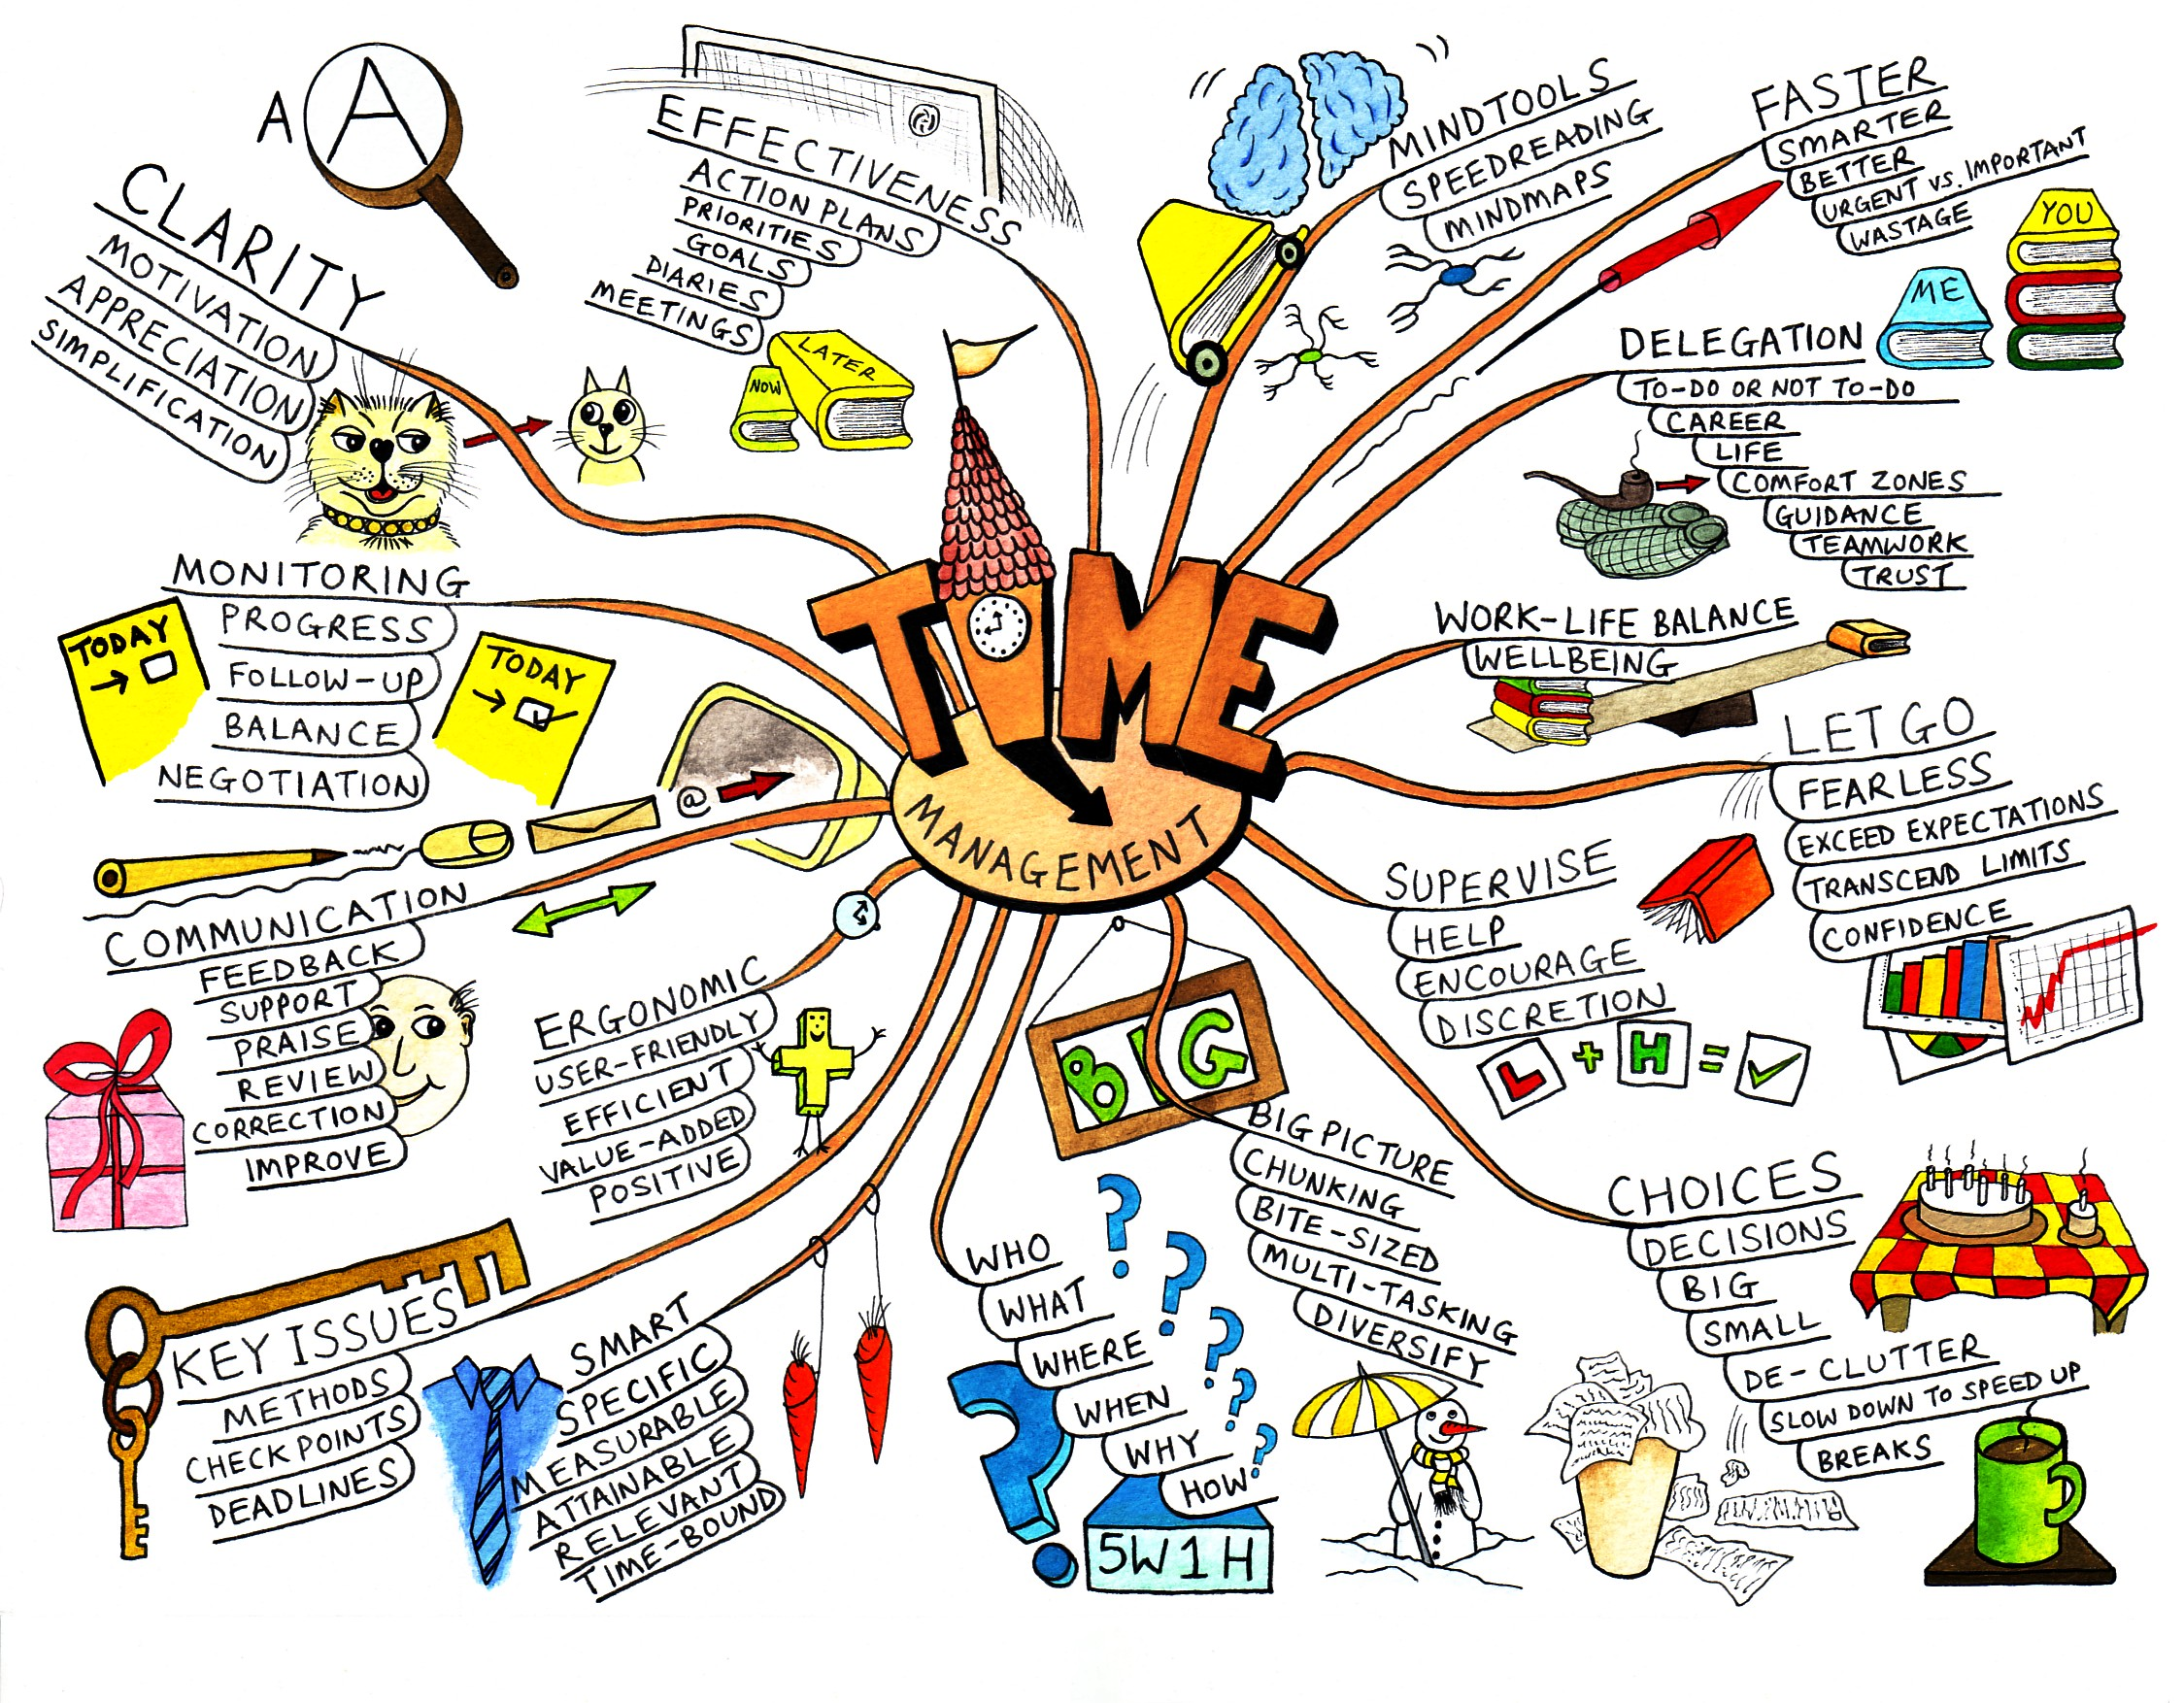
\includegraphics[width=\textwidth]{../resources/illustrations/mindmap}
  \caption{Exemple de carte mentale.}
\end{figure}

Ajoutons tout de même que les méthodes d'apprentissage qui résultent des résultats obtenus dans le domaine des neurosciences n'entrent pas forcément en opposition avec le constructionnisme. Nous somme convaincu par le fait que rester ouvert aux différentes sphères de la recherche permettra de développer de meilleurs approches concernant l'apprentissage et le système éducatif en général.